\ifx\boi\undefined\ifx\problemname\undefined
\providecommand\sampleinputname{}
\providecommand\sampleoutputname{}
\documentclass[polish]{templates/boi}
\problemlanguage{.pl}
\fi
\newcommand{\boi}{Bałtycka Olimpiada Informatyczna}
\newcommand{\practicesession}{Dzień próbny}
\newcommand{\contestdates}{27 kwietnia - 1 maja 2018}
\newcommand{\dayone}{Dzień 1}
\newcommand{\daytwo}{Dzień 2}
\newcommand{\licensingtext}{To zadanie jest objęte licencją CC BY-SA 4.0.}
\newcommand{\problem}{Zadanie}
\newcommand{\inputsection}{Wejście}
\newcommand{\outputsection}{Wyjście}
\newcommand{\interactivity}{Interakcja}
\newcommand{\grading}{Ocenianie}
\newcommand{\scoring}{Punkty}
\newcommand{\constraints}{Ograniczenia}
\renewcommand{\sampleinputname}{Przykładowe wejście}
\renewcommand{\sampleoutputname}{Przykładowe wyjście}
\newcommand{\sampleexplanation}[1]{Wyjaśnienie do przykładu #1}
\newcommand{\sampleexplanations}{Wyjaśnienie do przykładów}
\newcommand{\timelimit}{Limit czasu}
\newcommand{\memorylimit}{Limit pamięci}
\newcommand{\seconds}{s}
\newcommand{\megabytes}{MB}
\newcommand{\group}{Grupa}
\newcommand{\points}{Punkty}
\newcommand{\limitsname}{Limity}
\newcommand{\additionalconstraints}{Dodatkowe ograniczenia}
\newcommand{\testgroups}{
Zestaw testów dzieli się na kilka grup, każda jest warta pewną liczbę punktów.
Każda grupa składa się z jednego bądź większej liczby testów.
Aby otrzymać punkty za daną grupę, Twoje rozwiązanie musi przejść wszystkie testy z tej grupy.
Ostateczny wynik za zadanie jest liczony jako maksymalny wynik z pojedynczych zgłoszeń.
}



% \fi
% \newcommand{\boi}{Baltic Olympiad in Informatics}
% \newcommand{\practicesession}{Practice Session}
% \newcommand{\contestdates}{April 27 - May 1, 2018}
% \newcommand{\dayone}{Day 1}
% \newcommand{\daytwo}{Day 2}
% \newcommand{\licensingtext}{This problem is licensed under CC BY-SA 4.0.}
% \newcommand{\problem}{Problem}
% \newcommand{\inputsection}{Input}
% \newcommand{\outputsection}{Output}
% \newcommand{\interactivity}{Interactivity}
% \newcommand{\grading}{Grading}
% \newcommand{\scoring}{Scoring}
% \newcommand{\constraints}{Constraints}
% \renewcommand{\sampleinputname}{Sample Input}
% \renewcommand{\sampleoutputname}{Sample Output}
% \newcommand{\sampleexplanation}[1]{Explanation of Sample #1}
% \newcommand{\sampleexplanations}{Explanation of Samples}
% \newcommand{\timelimit}{Time Limit}
% \newcommand{\memorylimit}{Memory Limit}
% \newcommand{\seconds}{s}
% \newcommand{\megabytes}{MB}
% \newcommand{\group}{Group}
% \newcommand{\points}{Points}
% \newcommand{\limitsname}{Limits}
% \newcommand{\additionalconstraints}{Additional Constraints}
% \newcommand{\testgroups}{
% Your solution will be tested on a set of test groups, each worth a number of points.
% Each test group contains a set of test cases.
% To get the points for a test group you need to solve all test cases in the test group.
% }
\fi
\def\version{jury-1}
\problemname{Prąd przemienny}
Ferdynand bawi się w domu swoją zrobioną na zamówienie kolejką, która napełnia go wielką dumą.
Tor kolejki podzielony jest na $N$ segmentów połączonych w kółko, ponumerowanych $1, 2, \dots, N$
w kolejności zgodnej ze wskazówkami zegara. Segmenty są zasilane prądem za pomocą $M$ przewodów poprowadzonych
wzdłuż toru. Wzdłuż każdego segmentu biegnie co najmniej jeden przewód.

Ferdynanda zaczął nudzić pociąg, który nie robi nic więcej poza jeżdżeniem w kółko, więc
postanowił do każdego segmentu dodać przełącznik zmieniający kierunek jazdy, aby móc
aranżować wypadki i inne nieco bardziej ekscytujące scenariusze.
Jednak takie przełączniki też wymagają prądu. I to nie byle jakiego -- musi to być \emph{prąd przemienny.}
\footnote{Taka konstrukcja naprawdę działa w szwedzkich kolejach -- wszystkie przełączniki (,,växlar'') używają prądu przemiennego (,,växelström'').}


Ferdynand wymyślił, że doskonałą metodą uzyskania prądu przemiennego
będzie podłączenie przełącznika do dwóch źródeł prądu płynącego w przeciwnych kierunkach.
Każdy przewód przewodzi prąd wyłącznie w jedną stronę (zgodnie lub przeciwnie do wskazówek zegara),
lecz Ferdynand może wybrać w którą. Postanowił więc tak podobierać kierunki prądu w poszczególnych przewodach,
aby wzdłuż każdego segmentu biegł przewód przewodzący prąd zgodnie ze wskazówkami zegara oraz przewód przewodzący
w przeciwnym kierunku.

Potrafisz pomóc mu w tym zadaniu?

\vspace{2mm}
%\hspace*{2mm}
\begin{center}
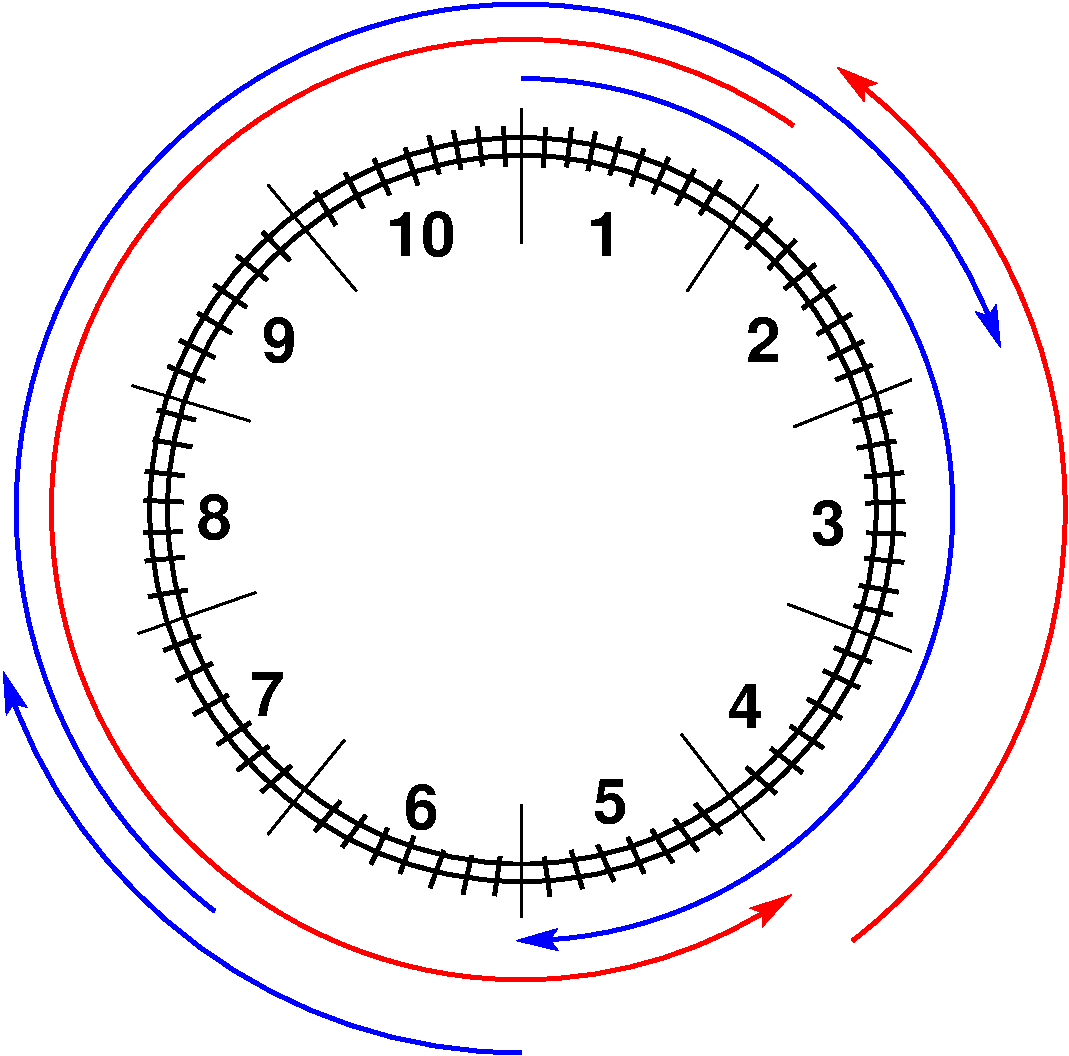
\includegraphics[width=0.5\textwidth]{alternatingfig.pdf}
\end{center}
\vspace{1mm}
{\em Rozwiązanie pierwszego testu przykładowego. Strzałki na zewnątrz toru przedstawiają przewody.
Kierunek i kolor strzałek oznacza kierunek, w którym dany przewód przewodzi prąd.
Odwracając kierunki wszystkich strzałek również uzyskamy poprawne rozwiązanie: \texttt{11010}.}

\newpage

\section*{\inputsection}
Pierwszy wiersz wejścia zawiera dwie liczby całkowite $N$ i $M$ oznaczające odpowiednio liczbę segmentów toru i liczbę przewodów.
Każdy z następnych $M$ wierszy zawiera dwie liczby całkowite $1 \le a, b \le N$ oznaczające przewód
biegnący przez segmenty $a, a+1, \dots, b$. Jeśli $b$ jest mniejsze niż $a$ oznacza to, że przewód
biegnie przez segmenty $a, \dots, N, 1, \dots, b$. W przypadku $a=b$ przewód pokrywa tylko jeden segment.

\section*{\outputsection}
Na wyjście wypisz pojedynczy wiersz zawierający $M$ znaków \texttt{0} lub \texttt{1}.
$i$-ty znak oznacza kierunek prądu płynącego przez $i$-ty przewód z wejścia -- $0$ oznacza kierunek
zgodny ze wskazówkami zegara, $1$ przeciwny. W~przypadku wielu możliwych rozwiązań wypisz dowolne z nich.

Jeśli nie da się tak pokierować prądu w przewodach, aby przez każdy segment biegł prąd w obu kierunkach, wypisz
,,\texttt{impossible}''.

\section*{\constraints}
\testgroups

\noindent
\begin{tabular}{| l | l | l | l |}
\hline
\textbf{\group} & \textbf{\points} & \textbf{\limitsname} & \textbf{\additionalconstraints} \\ \hline
  1     & 13     & $2 \le N, M \le 15$ & \\ \hline
  2     & 20     & $2 \le N, M \le 100$ & \\ \hline
  3     & 22     & $2 \le N, M \le 1000$ & \\ \hline
  4     & 19     & $2 \le N, M \le 100\,000$ & Dla żadnego przewodu nie zachodzi $b < a$. \\ \hline
  5     & 26     & $2 \le N, M \le 100\,000$ & \\ \hline
\end{tabular}
